\section{Testing the security measures}
This paragraph only deals with testing results obtained for the implementation of the \textbf{arpwatch} tool and the security measures taken in the context of the \textbf{arpwatch-clients} machine: results concerning the testing of the \textbf{DHCPv4} service were already shown in the corresponding paragraph.\\
Every sensitive file - scripts for monitoring tasks, so Python and shell scripts, and the \textit{arpwatch.log} file - were tested against escalation of privileges attacks by trying to tamper with them directly from the target machine through the \textbf{wtachdog} user logged in, with commands such as \textit{nano arpwatch.log} or \textit{vi arpwatch$_$shell$_$script.sh}, and while these files are actually readable, they cannot be modified by the user unless it executes these commands via \textbf{sudo} authentication, which requires the user itself to know a specific, not set by default password. The user itself cannot create other files without the aforementioned password, and cannot execute a reboot of the machine for the very same reason.\\
The user can execute without authentication only the monitoring scripts in the \textbf{arpwatch-clients} machine, and the only script that receives an input - \textit{scapySendPacket.py} - correctly performs input validation as shown by the trivial example in \textbf{Figure 9}.\\
\begin{figure}[htpb]
\centering
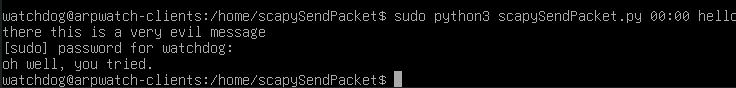
\includegraphics[width=0.8\textwidth]{inputValidation_pythonScript.png}
\caption[a]{Python Script executed with sudo rejecting an undesired input which is not found in the log file.}\label{fig:9}
\end{figure}

Furthermore, after logging out of the \textbf{watchdog} user in the \textbf{arpwatch-clients} machine, we verified the monitoring task is carried out as requested by the assignment by executing several ping commands - either directed to the internal router, or out of the LAN, or to the \textbf{arpwatch-clients} machine itself - in the \textbf{kali} machine and capturing all the packets on its interface \textbf{eth0}, and we observed the new station being registered by \textbf{arpwatch} and then notified through the packet sent by the script. As a final step, we changed multiple times the MAC address and the IP address of the \textbf{kali} machine, observing the packets sent to it by \textbf{arpwatch} and advising it of \textbf{flip$-$flop} activity, IP address changed or MAC address changed.\\
A trivial example of the monitoring task being executed correctly is shown in \textbf{Figure 10}.\\
\begin{figure}[htpb]
\centering
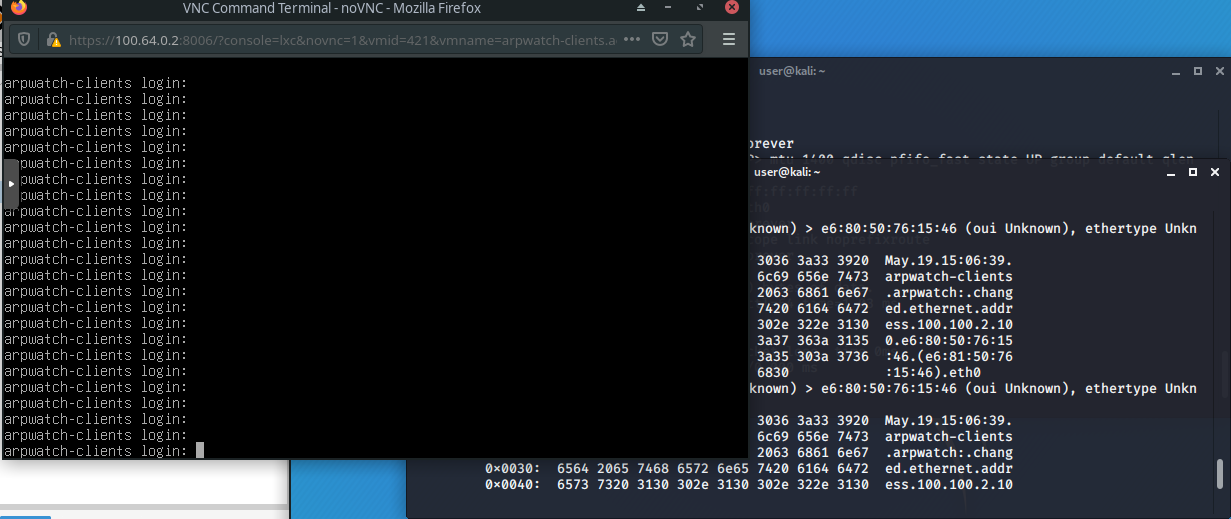
\includegraphics[width=1\textwidth]{detection_while_logged_out.png}
\caption[a]{Arpwatch logged out still sending the desired detection packets to the target.}\label{fig:9}
\end{figure}
